\documentclass[reviewcopy]{elsart}
\usepackage{ifpdf}
\usepackage{graphicx,natbib,amssymb,lineno}
\usepackage{epsfig}
\ifpdf
\usepackage[%
  pdftitle={Instructions for use of the document class
    elsart},%
  pdfauthor={Simon Pepping},%
  pdfsubject={The preprint document class elsart},%
  pdfkeywords={instructions for use, elsart, document class},%
  pdfstartview=FitH,%
  bookmarks=true,%
  bookmarksopen=true,%
  breaklinks=true,%
  colorlinks=true,%
  linkcolor=blue,anchorcolor=blue,%
  citecolor=blue,filecolor=blue,%
  menucolor=blue,pagecolor=blue,%
  urlcolor=blue]{hyperref}
\else
\usepackage[%
  breaklinks=true,%
  colorlinks=true,%
  linkcolor=blue,anchorcolor=blue,%
  citecolor=blue,filecolor=blue,%
  menucolor=blue,pagecolor=blue,%
  urlcolor=blue]{hyperref}
\fi

\renewcommand\floatpagefraction{.2}
\makeatletter
\def\elsartstyle{%
    \def\normalsize{\@setfontsize\normalsize\@xiipt{14.5}}
    \def\small{\@setfontsize\small\@xipt{13.6}}
    \let\footnotesize=\small
    \def\large{\@setfontsize\large\@xivpt{18}}
    \def\Large{\@setfontsize\Large\@xviipt{22}}
    \skip\@mpfootins = 18\p@ \@plus 2\p@
    \normalsize
}
\@ifundefined{square}{}{\let\Box\square}
\makeatother

\def\file#1{\texttt{#1}}

\pagestyle{plain}
\begin{document}

\begin{frontmatter}
\title{Generating MDA's Platform Independent Model using URDAD}

\author{Fritz Solms and Dawid Loubser}
\address{Solms Training and Consulting CC, PostNet Suite 237, Private Bag X9,
Melville, 2109, Johannesburg, South Africa.}

\ead{fritz@solms.co.za}
\ead[url]{http://www.solms.co.za/}

\begin{abstract}
  This paper formulates a set of minimal requirements for the
  Platform Independent Model (PIM) of the Model Driven Architecture
  (MDA). It then defines the Use Case, Responsibility Driven Analysis and
  Design methodology (URDAD) which provides a simple, algorithmic
  design methodology generating a PIM satisfying the specified PIM
  requirements.
\end{abstract}

\begin{keyword}
URDAD, design methodology, model driven development, MDA, business
process design
\end{keyword}
\end{frontmatter}

%%%%%%%%%%%%%%%%%%%%%%%%%%%%%%%%%%%%%%%%%%%%%%%%%%%%%%%%%%%%%%%%%%%%%%%%%%%%%%%%%%%%%%
%%
%%                             Refereee concerns
%%
%%  Referee 1:
%%  ==========
%%    - support with real-life experiences
%%        => addressed in a new subsection entitled "Real-life experiences with URDAD"
%%    - differences betw URDAD & stepwise refinement
%%        => added "Analysis and design methodologies" subsection of introduction to address this
%%    - how to fix levels of granularity in practice
%%       => The second and third paragraph of the section titled "The analysis phase of URDAD"
%%          has been rewritten to address this. The concepts are further enforced at the start
%%          of the analysis section of the example
%%    - major: review related MDA work, refinement processes, design & developments processes
%%        => partially addressed by additions to the "MDA-based development methodologies"
%%           subsection of introduction
%%    - include transformation viewpoint: process may configure & control set of transformation tasks
%%        => partially alluded to in "Analysis and design methodologies" subsection of introduction
%%        => discussed in a new model transformations section
%%    - what about intermediate PIMs (human comprehensible, ...)
%%        => We don't envisage intermediate PIMs. Humans should preferably have to deal with
%%           only a single set of artifacts. We would, however, see the benefit of multiple levels
%%           of PSMs at times. The fact that mappings typically involve a series of intermediate PSMs
%%				 is alluded to in the added section on model transformations
%%    - larger figures
%%    - last section before chapter 5 is unclear
%%        => has been rewritten
%%    - footnote on p17 too stand-alone
%%        => The footnote has been replaced by an in-text paragraph and the content has been
%%				reformulated in a more understandable way
%%
%%  Referee 2:
%%  ==========
%%    - case studies
%%        => referred to in the new subsection entitled "Real-life experiences with URDAD"
%%    - illustration figures used at SOMET'07 omitted - why?
%%        => have added the figure for a typical model-driven development process and for the collaboration context.
%%    - integrate issues mentioned in SOMET'07 to complete paper
%%        => have done so
%%    - show integration betw business process design, IT, project performance, business performance
%%      with reference to vendor-independent, business management knowledge base.
%%			=> this concern has not been dealt with in depth - it is partially alluded to in the added section
%%				"MDA-based development methodologies".
%%    - what is good process design from different points of view (PM, management, user, implementor, ...)
%%			=> this issue has been addressed by additions to the last paragraph of the section titles "Design quality drivers"
%%    - compare more to existing approaches
%%			=> addressed by additions to the "Analysis and design methodologies" subsection of introduction
%%    - transition across levels of granularity discussed in too abstract terms
%%       => this entire section has been rewritten in less abstract terms.
%%    - how to ensure compatibility betw outputs of technology neutral BP design & implementation?
%%         => partially discussed in the URDAD meta-model as mentioned in model transformations section
%%    - business processes need to be employed in environment ensuring certain qualities.
%%      How addressed?
%%			  => Discussed in a new section titled "Quality of service"
%%         => Needs/requirements for this mentioned in inputs for implementation mappings
%%    - How is minimal structure achieved?
%%         => Explained in the last paragraph added to the section titled "The design phase of URDAD".
%%    - Need repository to trace across levels of granularity?
%%         => Added a subsection to the Methodologies section titled "Navigating the PIM".
%%    - How to discover appropriate domains of responsibility? How to ensure no overlaps?
%%         => Rewrote first paragraph of "The design phase of URDAD" to explain this better.
%%    - Justify usage of diagrams (why minimal, complete set and why in that order?) Why not other
%%      like component/composite structure diagrams for system structure, ...
%%         => Added a subsection entitled "Choice of UML diagrams" to the modeling languages section.
%%    - Not all figures referred to in paper (e.g. figure 8)
%%          => fixed
%%    - Include how to evaluate URDAD based design
%%			=> addressed in new section "Evaluating URDAD based design"
%%
%%  Referee 3:
%%  ==========
%%    - how to guarantee technology mapping automation?
%%        => partially addressed by the new model transformations section.
%%    - clearer statement of original contribution of this work
%%        => added "Analysis and design methodologies" subsection of introduction to address this
%%    - add : to eol before start of bulleted lists
%%    - shorten figure captions
%%        => done
%%    - check typo/language comments (many)
%%        => done
%%
%%
%%
%%%%%%%%%%%%%%%%%%%%%%%%%%%%%%%%%%%%%%%%%%%%%%%%%%%%%%%%%%%%%%%%%%%%%%%%%%%%%%%%%%%%%%%

\section{Introduction}

The vision of model driven development (MDD)
\cite{schmidt:modelDrivenEngineering,stahl:mdsd}
even predates the definition of the Unified Modelling Language (UML); yet it
has historically been implemented with little success. With a cleaner separation of
architecture from design as envisaged by the Object Management Group's (OMG),
Model Driven Architecture (MDA) \cite{siegel:developingInMDA,frankel:enterpriseMDA}
together with semantically richer modelling languages like UML 2.x and stronger
tools support for MDD, the interest in MDD has increased considerably.

Yet there are a number of open issues which hold back the widespread adoption of MDD.
The first issue is the lack of a clear definition on what needs to be included in the
Platform Independent Model (PIM). Braek and Melby \cite{braek:modelDrivenServiceEngineering}
define a minimal requirements without specifying precisely the required components
for the PIM. This paper attempts to specify more concretely the artifacts which should
be included in a PIM.

The second issue is the lack of standards available to define the implementation architecture
and technologies required for the implementation mapping. This aspect is then often addressed in
a tool specific way like, for example, the cartridges approach of Andro-MDA. Usually this aspect
is further simplified by MDA tools supporting a specific set of reference architectures like
Java-EE, CORBA, CCM, JBI/SOA or Microsoft.Net.

The third issue slowing down the wide-spread adoption of MDA is the virtual lack of
a well defined, practical analysis and design methodology together with a
precise definition of the inputs and outputs
including the artifacts which must be included in the specification of a PIM.
which must be produced to define a required with specified inputs and outputs.

In this paper we will try and formulate some steps towards addressing the first
two issues. We will formulate some requirements for the PIM and will present
the Use-Case, Responsibility Driven Analysis and Design (URDAD)
\cite{solms:urdad}, a simple, algorithmic analysis and design methodology
which can be used by domain experts such as business analysts to generate the
PIM. The domain experts need not have an understanding of the implementation
architecture and technologies.

%--------------------------------------------------------------------

\subsection{Analysis and design methodologies}

Historically, URDAD has grown out of Responsibility Driven Design (RDD)
methodology pioneered by Rebecca Wirfs-Brock and Brian Wilkerson (see
\cite{wirfs-brock:responsibilityDrivenApproach},  and
\cite{wirfs-brock:objectDesign} \cite{wirfs-brock:designSimplicity}) and has
been influenced by the approaches of step-wise refinement \cite{wirth:stepWiseRefinement}
and top-down design \cite{martin:agileSoftwareDevelopment}.

But, while all of these are design approaches, URDAD provides an algorithmic
analysis and design methodology with the following characteristics:
\begin{enumerate}
  \item Both, requirements and design are step-wise refined.
  \item URDAD specifies the steps of the design methodology with
			well-defined inputs and outputs for each step, making the process repeatable
			and predictable.
  \item Generation of services contracts for the service providers required at any
			level of granularity enforcing a technology-neutral approach as well as
			pluggability and testability at any level of	granularity.
	\item Work flow logic at any level of granularity is factored out of the service
			providers for that level of granularity, enforcing decoupling of role players
			across levels of granularity.
	\item URDAD provides an explicit approach to fixing the levels of granularity.
   \item URDAD explicitly aims to generate a technology and architecture neutral design
			representing MDA's PIM.
\end{enumerate}

One of the benefits of having a standard design methodology generating a set of
predictable artifacts for the PIM, is that it simplifies the mapping from the platform
independent model (PIM) to the platform specific model (PSM), i.e.\ the methodology defines
standard set of source elements for the model transformations.

%------------------------------------------------------------------------------

\subsection{MDA-based development methodologies}

URDAD is usually embedded within an iterative realization or development process. Reviews of some
MDA-based development methodologies can be found in \cite{bercovici:businessArchitectureToSoa}
A typical model driven development process is shown in figure \ref{fig:developmentProcess}. 
Note that the technology neutral business process design is performed by business analysis. 
The technical team comprising both, architecture and implementation (development), 
is responsible for the realization of the business process within the chosen architecture and technologies.

\begin{figure}
  \centering
  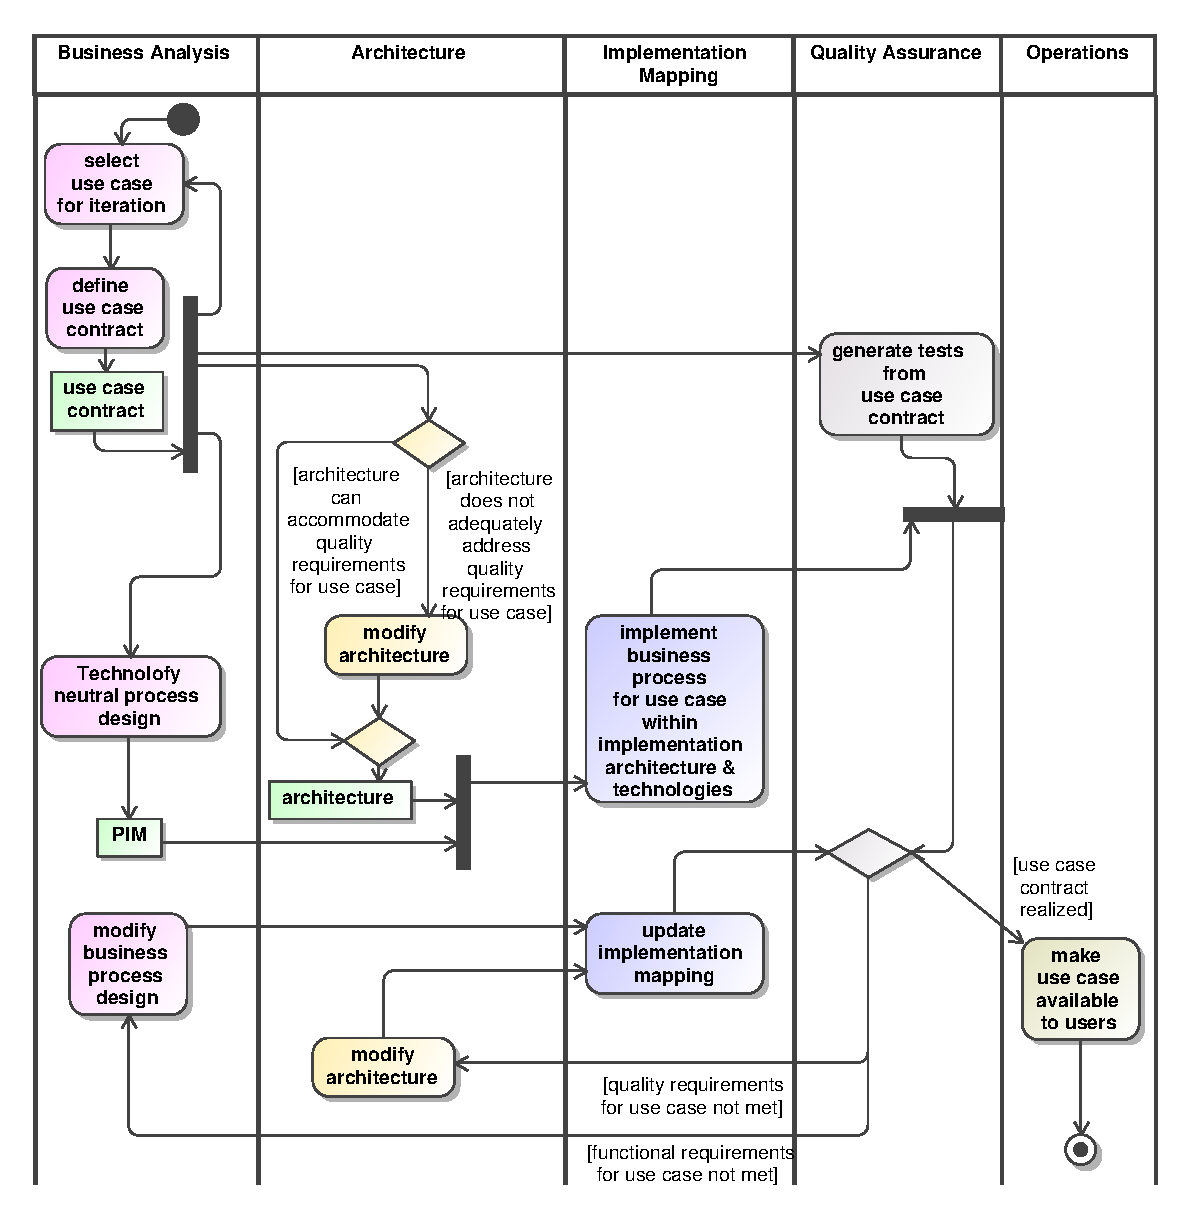
\epsfig{file=developmentProcess.eps, scale=0.6}
  \caption{Outline of a model driven development process.}
  \label{fig:developmentProcess}
\end{figure}

After passing quality assurance and actual deployment, operations takes over the management of the
business process execution.

%-------------------------------------------------------------------------------

\subsection{Real-life experiences with URDAD}

URDAD has been developed and taught to both business analysts and software designers since 2002.
More than a dozen of companies have been and are using URDAD for their technology neutral analysis
and design methodology. Some of these have decided to enforce the URDAD methodology as an organization
wide standard. Examples of such companies include
\begin{itemize}
  \item {\em Strate} (http://www.strate.co.za), the authorized Central Securities Depository (CSD) for the electronic settlement of all financial instruments in South Africa.
	\item {\em AllCare Administrators} (http://www.allcare.co.za), a medical aid administrator, and
	\item {\em Multichoice} (http://www.multichoice.co.za), the premier digital media provider in South Africa.
\end{itemize}
Strate's experiences with URDAD have been partially documented in \cite{klopper:compareSoftwareMethodologies}.

The main reasons for standardizing on URDAD typically include
\begin{itemize}
  \item higher productivity achieved through the algorithmic process and the separation of technical concerns,
  \item standardized outputs of the analysis and design process with improved quality and consistency, and
  \item the benefits of having business processes documented in a technology neutral way.
\end{itemize}

Core difficulties often experienced include
\begin{itemize}
  \item a resistance to adopting UML for business process documentation, and
  \item challanges around separating the business processes from the currently employed technologies, and
  \item insufficient understanding of the methodology leading to inconsistent and low-quality results.
\end{itemize}


\section{Model-Driven Development (MDD)}


{\em Model Driven Development} (MDD) or its more generic form, Model Driven
Engineering (MDE),
\cite{selic:pragmaticsOfModelDrivenDevelopment,schmidt:modelDrivenEngineering, france:mddUsingUml2}
is increasingly gaining the attention of both research communities and the software development industry.

In MDD one aims to capture and maintain the business processes within abstract models,
which are then mapped onto (typically software-based) implementations. The
aim is to simplify the development and maintenance of the business processes,
as well as to facilitate automation via techniques such as model execution, model transformation 
or code generation.

The {\em Object Management Group} (OMG) promotes the Model Driven Architecture
(MDA) \cite{pastor:mdaInPractice,siegel:developingInMDA,frankel:enterpriseMDA,
stahl:mdsd}
as a standard framework for MDD. It proposes the development of a
technology neutral model, the {\em Platform Independent Model} (PIM) which is
then mapped onto one's choice of implementation architecture and technologies
via standard model transformations defined for such technologies. One of the
core benefits envisaged by MDA is that the PIM will be able to survive
technology and architecture changes \cite{siegel:developingInMDA}.

\subsection{Quality of service}

Business processes need to be deployed within an environment ensuring certain qualities.
It is the responsibility of architecture to ensure that the infrastructure into which
the business processes are to be deployed will provide the required qualities
\cite{bass:softwareArchitecture}.

URDAD thus assumes the orthogonality of the technology neutral business process design and
the implementation architecture with the former addressing the functional requirements and
the latter addressing the non-functional or quality requirements.

\subsection{Model transformations}

In a model driven approach, the platform independent model is taken through one or
more model transformations which map the technology neutral business process specification
contained in the PIM onto a series of intermediate Platform Specific Models (PSMs)
and ultimately onto a concrete, deployable implementation, the Enterprise Deployment Model (EDM).
The OMG has defined for this the QVT (Queries/Views/Transformations) \cite{omg:qvt}
which is an extension of the Object Constraint Language (OCL) and contains three domain
specific transformation languages. Other languages used to specify model transformations include
the Model Transformation Language (MTL), the ATLAS Transformation Language (ATL) as well as domain-neutral
languages like the XSLT and Java.

The inputs for the implementation mappings are
\begin{enumerate}
  \item the technology neutral analysis and business process design in the form of a PIM including
			the quality requirements for the deployed services, and
  \item the Platform Description Model (PDM) specifying the implementation architecture
			and technologies including the presentation layer infrastructure (e.g.\ Struts),
			the integration infrastructure, the component/services hosts, the persistence
			infrastructure, ...
\end{enumerate}
In order to perform a model transformations one requires the understanding of the meta models of both,
the source language as well as the target language.

URDAD defines a meta model for the
structure of the PIM. The semantics required for the meta-model is defined in a UML profile for URDAD.
Part of the PIM are the service provider contracts with the quality of service requirements. These are
specified using OMG's {\em UML Profile for Modeling Quality of Service and Fault Tolerance Characteristics
and Mechanisms} \cite{omg:umlProfileQos}. Having a well-defined meta-model for the PIM significantly
simplifies the definition of model transformations required to generate the PSMs and EDM.

The weak aspect of the source domain is usually the specification for the PDM.
Due to a lack of standards around the specification of the PDM, MDA tools often support only
mappings onto certain specific reference architectures/platforms like Java EE and Microsoft.Net
with only limited control over the parameters of the defined architecture. Alternatively
or additionally they enable one to specify the PDM indirectly through a set of transformation
elements.




\section{Requirements for the resultant PIM}
\label{sec:pimRequirements}

Braek and Melby \cite{braek:modelDrivenServiceEngineering} define a set
of minimal requirements for the PIM. In particular, they specify that the
PIM should be
\begin{itemize}
  \item platform-independent, and hence technology neutral,
  \item comprehensible and maintainable by humans,
  \item analytical in order to facilitate implementation verification and
comparison, and
  \item domain realistic in that it can realistically model the real world.
\end{itemize}

The people or systems performing the implementation mapping of the
technology neutral business processes would obtain the PIM together
with a specification of the enterprise architecture, i.e.\ the organizational
and systems infrastructure within which the business processes are to be
deployed. The PIM and architecture specification should be sufficient
in the sense that no further important
decisions should have to be made during the implementation mapping.

In principle, the PIM should be executable within an executable environment
similar to interpreted or platform-independent programming languages executing
in runtime environments. Such environments could be used for model testing. 
Testing frameworks could generate mock services providers that realise the externally
visible pre- and post-conditions in the case of the model containing contracts without
the corresponding business processes to realise them (such as in the case of external
service providers).

%------------------------------

\subsection{PIM components}

In order to contain sufficient information for an implementation mapping onto
some externally defined architecture, 
URDAD requires that the PIM must contain the following artifacts:
\begin{description}
  \item[Services contracts] For each level of granularity, the services
 	contracts for each responsibility domain at that level of
	granularity. The services contracts must specify the services which
	any service provider implementing the services contract needs to
	provide together with the inputs, outputs, pre- and post-conditions, and
	quality requirements for each service.
	Examples of services contracts include services contracts for 
	\begin{itemize}
	  \item internal service providers for which lower level
		business processes
		realising these services contracts are specified at a lower
		level of granularity,
	  \item external services providers to whom
		certain responsibilities are out-sourced,
	  \item responsibility domains which are
		realized by off-the-shelf systems or systems developed by
		external development partners,
	  \item user contracts, specifying what is required from the users of
		services, and
	  \item base processing elements performing certain basic computational
		services which obtain some input and transform it to some
		output.
	\end{itemize}

  \item[Business process specifications] The specification on how a business
	process at any level of granularity is assembled from the services
	defined within the services contracts for that level of granularity.	

  \item[Request construction] The PIM must contain the specification on
	how the information required for a service request is assembled
	from the currently available information.

  \item[Data structure specification] The model must contain the data structure
	requirements in a technology neutral way.
\end{description}

%---------------------------

\subsection{PIM boundaries}

An important consideration during the modelling process is the definition of the
boundary of the PIM, i.e.\ which service providers will be realized as part of the
system, versus the service providers which will be treated as external to the
system (such as services provided by business partners).

The architecture specifies the organizational and systems infrastructure which
will host the business processes. It will also need to specify the boundaries of
the organization, i.e.\ what is within and what is outside the scope of the
organization, as well as the responsibilities which are to be hosted within
off-the-shelf systems and systems developed by external development partners
and in-house developments.

It is thus the architecture which will enable one to decide which
services contracts fall within the scope of operations for the organizations and
which will be out-sourced to external service providers or system vendors. For
those responsibility domains which are outside the scope of the organization,
the PIM will only specify the services contracts and not the lower level
business processes employed to realise these services contracts.


\section{The URDAD methodology}

The aim of URDAD is to provide a simple step-for-step, use-case driven analysis
and design algorithm which can be used by domain experts (e.g.\ business
analysts) to design processes (e.g.\ business processes) in a technology neutral
way. The resultant PIM is meant to be
mappable onto different implementation architectures and technologies.

%==================================================

\subsection{Methodology Requirements}

The outputs of the URDAD design methodology should comply to the PIM
requirements discussed in section \ref{sec:pimRequirements}. In addition the
methodology should be usable, simplifying the design
process and ensuring the consistency and quality of its outputs,
i.e.\ the methodology should satisfy the Berard requirements
\cite{berard:whatIsMethodology}.

In order to judge the quality of the outputs, one needs to specify the criteria
along which the quality of a design is judged.
Desired design qualities include simplicity
\cite{wirfs-brock:designSimplicity}, clean layers of granularity
\cite{martin:agileSoftwareDevelopment, artus:soaRealization},
flexibility and maintainability
\cite{hordijk:maintainabilityFactors,misra:drivingMaintainableDesign},
a high level of reusability \cite{lenz:softwareReuse}, and
testability across layers of granularity \cite{voas:softwareTestability}. In
addition, we require that the resultant design complies to the PIM
requirements specified in section  \ref{sec:pimRequirements}.

\begin{figure}
  \centering
  \epsfig{file=designActivities.eps, scale=0.6}
  \caption{Desired design qualities.}
  \label{fig:designActivities}
\end{figure}

Generating a design with the desired design qualities provides core business
benefits including improved flexibility and time-to-market,
improved reliability and the ability of business (instead of technology)
taking ownership of the business process designs.

%=================================================

\subsection{Design quality drivers}

We need to define an analysis and design algorithm which not only generates a
PIM which satisfies the PIM requirements, but one which also will exhibit
the desired design qualities.

Aiming to explicitly realize the design qualities is not necessarily an advisable
approach. For example,  one would often not want to
consciously design for, for example, re-usability. Such an approach would
necessitate that one would need to envisage potential future re-use scenarios.
This is not only a difficult task, but it also results in significant cost
overheads with uncertain returns and increased complexity. Instead one would want
to generate the simplest design solution which addresses the current requirements,
and achieve the qualities through a sound design process.

URDAD specifies a set of design activities which will drive out the desired
design qualities (see figure \ref{fig:designActivities}).
For example, the activities of enforcing the single
responsibility principle \cite{wirfs-brock:objectDesign,
wirfs-brock:responsibilityDrivenApproach}, decoupling via contracts
\cite{meyer:designByContract} and localizing the business process information
for any service at any level of granularity, one promotes reusability across
levels of granularity.

But, enforcing a contracts based approach not only drives re-usability, it also
improves simplicity and understandability (it is often sufficient to understand the
services contract without having to understand how the services contract is
realized) as well as testability (only once we have a solid services contract are we
really in a position to define service provider tests).

Figure \ref{fig:designActivities} shows the dependencies of the design qualities on
standard design activities enforced within the URDAD methodology. The details of
how these design activities generate a design with the desired design qualities
can be found in \cite{solms:urdad}.

Different role players may require, of course different design qualities. Business
management has indirectly an interest in all of these design qualities since they
all contribute to generating business value. They have a particular interest in
having technology neutral business process documentation across levels of granularity.
Project Management is particularly
concerned about traceability for estimation purposes and testability for status
reporting purposes. Business analysts require the simplicity and understandability
in order to be able to effectively work with business processes. Furthermore, clean
layers of granularity makes it easier for business analysts from different responsibility
domains to collaborate on a single business model. Implementors would like the freedom
to choose the implementation technologies, a high level of reuse and benefit from traceability,
testability and simplicity and understandability of the design.

%=================================================

\subsection{Analysis and technology-neutral design across levels of granularity}

URDAD is based on the view that both, analysis and design need to be done
across levels of granularity, i.e.\ that a single analysis phase generating
the functional requirements for a use case across levels of granularity
is not desirable. UML itself supports functional requirements across
levels of granularity via use case trees
with lower level functional requirements linked to higher level functional
requirements via {\em include} and {\em extend} relationships.
However, the analysis
and business process design across levels of granularity usually requires
business knowledge from different specialist domains and is hence often
performed across business analysts of various departments
contributing at different levels of granularity.

Furthermore, in the context of technology neutral design, the decision on
whether a particular domain of responsibility is to be hosted within the
organization or whether it is to be outsourced to external service providers is
only made when the implementation architecture is specified.

A technology neutral design methodology should thus support analysis and design
across levels of granularity, i.e.\ an analysis and a design phase for each
level of granularity.


%=================================================

\subsection{URDAD steps}

The steps of the URDAD methodology are shown in the first two swim lanes of
figure \ref{fig:methodology} while the implementation swim lane shows the
standard MDA steps for mapping the PIM onto an implementation.

\begin{figure}
  \centering
  \epsfig{file=methodology.eps, scale=0.6}
  \caption{The URDAD methodology.}
  \label{fig:methodology}
\end{figure}

The process is iterative around use cases and incremental across levels of
granularity. Note that for each level of granularity there is both, an analysis
as well as a design phase. The output of the analysis phase is the use
case contract the functional and non-functional requirements for the use
case. The output of the design phase is the PIM for that level of
granularity containing the services contracts for the service providers
required for that level of granularity and the business process assembled
from these services.

%------------------------------------------------------

\subsubsection{The analysis phase of URDAD}

URDAD, like many other design and software development methodologies is use
case driven. The first step in the analysis phase is to identify
all the stake holders who have an interest in the use case and who will
potentially specify requirements for the use case.

During the second URDAD step one identifies the functional requirements for each stake
holder. It is in this early stage that the level of granularity is fixed by only including
direct functional requirements (i.e.\ not lower level functional requirements of functional
requirements). The lower level functional requirements will be addressed when capturing
the functional requirements for the lower level use cases/services.

In practice, one often tends to go too fine grained too quickly. This problem can be addressed
by explicitly checking whether
\begin{itemize}
  \item some functional requirements can be seen as lower level details of others,
  \item assessing whether some functional requirements can be grouped into a higher
			level functional requirement.
\end{itemize}

For the first level of granularity, one may need to define the user work flow
showing the sequences of messages exchanged between the user and the subject
for the various scenarios. When coming to lower levels of granularity, the
user work flow is already defined via the dynamics at the higher level of
granularity.

The next step is to specify the stake holder requirements around the value
(data) objects exchanged between the user and the service provider. As one
designs the business process across levels of granularity, one will identify
further information which is required and one will feed the appropriate
data structure elements into these data objects.

Finally one needs to formally specify the pre-conditions (the conditions under
which the service provider may refuse the service without breaking the
contract), the post-conditions (the conditions which need to be satisfied after
a successful completion of the use case) and the quality requirements (the
non-functional requirements like scalability, reliability, security, and
performance requirements).

The post-conditions are a formalization of the client's functional requirements,
i.e.\ each functional requirement placed by the client will be formally refined
by defining a testable post-condition.

The functional requirements, user work flow specification, data object requirements
together with the pre- and post-condition and quality requirements define the
use case contract.

%------------------------------------------------------

\subsubsection{The design phase of URDAD}

The first two steps of the design phase are those of grouping functional
requirements into responsibility domains and assigning them to services
contracts. For this we need to ask ourselves what domain is ultimately
accountable for a particular service, without concerning ourselves whether,
at lower levels of granularity the service will touch other domains of
responsibility. That will be addressed when we get to these levels of
granularity. It is thus not essential to ensure that
there is no overlap between domains of responsibility as
lower level functional requirements will be assigned to the appropriate responsibility
domains and ultimately to the service providers assigned to these domains of responsibility.


The responsibility identification and allocation steps enforce the single responsibility principle, the
contracts based approach and by locking into services contracts instead of
classes or objects, also the technology neutral aspect of the design.


The user itself may have to address certain responsibilities. If that is the
case, URDAD will also introduce a services contract for the user, specifying
formally the user responsibilities for the use case.

Having introduced services contracts for the responsibility domains to
be addressed for the use case, one now specifies how the business process is
assembled across the services provided by the services providers realizing these
services contracts.

Finally one projects out the collaboration context which shows the minimal structure
required to support the business process for the current level of granularity. Note
that the entity objects are also populated as information is required within a business
process. In this way URDAD aims to ensure that the design only has those structural
elements which are required for the execution of the business processes realizing the
stake holder requirements.

%------------------------------------------------------

\subsubsection{Transition to next lower level of granularity}

In order to go to the next lower level of granularity, one
selects one of the service providers from the current level of granularity
as new subject. The services become the use cases for the analysis phase
of this level of granularity. One now repeats the process by first identifying
the stake holders who have an interest in this lower level service or use case,
and subsequently their functional requirements.
One thus repeats the steps of the analysis and design phase for this lower
level of granularity, omitting the user work flow specification as this is
provided by the previous (next higher) level of granularity.

%------------------------------------------------------

\subsubsection{Lowest level of granularity}

The lowest level of granularity is reached if either a particular domain
of responsibility is outsourced, or if the functional requirements need not be
refined any further. In either of these two cases one ends with a services
contract specifying pre- and post-conditions (using the OCL) and quality
requirements for the services.

Low level services which perform simple transformations or calculations are
fully specified via post-conditions specified in OCL, i.e.\ the post-conditions
have sufficient information in order for their implementation to be autogenerated.

\subsection{Navigating the PIM}

UML tools enable one to conveniently navigate across the views within a particular level of granularity and to traverse across levels of granularity. This is further simplified
by stereotyping the various model elements using the URDAD UML Profile.

%---------------------------------------------------------

%\subsection{The URDAD meta-model}  ################################

%The URDAD meta-model defines a set of standard artifacts. The semantics for these artifacts
%is introduced in a UML profileintroducing the following concepts:
%\begin{itemize}
%  \item {\em :} Stake-holder, User, Service-provider, Observer, Entity, Services-contract,
%			Workflow-controller.
%  \item {\em Relationships:} Service for use case, Activity-for-service.
%  \item {\em Diagrams:} Functional requirements, user work flow specification,
%			services contract specification, responsibility allocation, business.
%			process specification (either sequence or activity diagram).
%\end{itemize}

\section{URDAD and Modeling Languages}

Even though URDAD has been largely used in conjunction with the Unified Modeling Language (UML),
it is not locked into using any particular modeling language. In order for a modeling language
to be usable with the URDAD design methodology, it must have sufficient semantics to be able to
document the PIM. In particular, it requires support for
\begin{itemize}
  \item technology neutral business process modeling,
  \item services contracts,
  \item technology neutral data structure modeling,
  \item decomposition of services across levels of granularity, and
  \item declarative specification of how one data object is constructed from other data objects.
\end{itemize}

In addition the language should generate a semantically sound model which enforces consistency
across the statements made within the modeling language. Finally, it is desirable that any
modeling language used for URDAD is extensible in order to accommodate any additional semantics
required for MDD.

%----------------------------------------------
\subsection{URDAD and UML}

The Unified Modeling Language, UML, provides most modeling elements required by
URDAD. In particular, it supports
\begin{itemize}
  \item technology neutral business process design using sequence and
	activity diagrams,
  \item the specification of services contracts using UML interfaces together
	with the Object Constraint Language (OCL),
  \item technology neutral data structure specification using UML class diagrams, and
  \item the declarative specification of data object construction is done using OCL.
\end{itemize}

In addition, UML supports an underlying object model which ensures consistency
and semantic coherence across diagrams. It also has an extension mechanism,
stereotyping, which supports the introduction of refined concepts based on the
base concepts provided by UML.

One of the issues we have experienced with UML is that it does not have a convenient
notation for the concept of a service and for specifying dependencies between services.
The closest there is in UML, is the use case diagram where a use case is often interpreted
as {\em a service of value} and dependency between services is documented using
{\em include} and {\em extend} relationships. However, these use cases would still have to
be formally tied up to the services used in sequence and activity diagrams.
In URDAD services are formally linked to use cases via a realization relationship.

\subsubsection{UML adoption for technology neutral business process design}

Business analysts have been slow in adopting UML for technology
neutral business process design. This can be largely attributed to
the complexity of the UML, the perception that UML is largely useful for
modeling software systems, and the lack of simple design methodology which
provides business analysts guidance in using UML for technology neutral
business process design.

\subsection{Choice of UML diagrams}

URDAD aims to make it more feasible for business analysts to use UML by requiring
that only 4 of the 13 UML diagrams are used together with OCL constraints specification.
For the analysis phase, URDAD requires one use case diagram for the functional requirements, a sequences diagram for the user work flow, and a class diagram for the services contract.
For the design phase URDAD requires a further use case diagram for the responsibility
identification and allocation, a sequence diagram for the success scenario, an
activity diagram for the full business process specification and a class diagrams for the
collabaration context. URDAD thus mandates the use of only four of the thirteen UML diagrams.

This is a minimal, yet sufficient set of diagrams. Implementation mappings are ultimately done from the services contracts (with OCL
base pre- and post-conditions), the sequence and activity diagrams and the collaboration
context.

Communication diagrams provide an alternative view to the information contained in sequence diagrams, but are much less accessible to business analysts.
URDAD envisages the use of composite structure diagrams and component and deployment diagrams are really only for platform specific models. State charts are not used since URDAD effectively churns out a design with stateless service providers, i.e.\ a design which is largely in the spirit of services oriented approaches. Since timing diagrams are essentially a merger between
sequence diagrams and state charts, they are not used either. Interaction overview diagrams are not used as they typically traverse levels of granularity. Package and object diagrams are only
used implicitly.

%----------------------------------------------

\subsection{URDAD and BPMN}

Even though BPMN has reasonable support for business process specification
across levels of granularity (via compound activities), it does not currently
contain sufficient semantics for technology neutral business process design in
the spirit of model driven development. In particular, BPMN does not currently
have support for

\begin{itemize}
  \item solid services contracts specification, or for

  \item data structure specification (BPMN only supports artifacts whose
	structure is to be specified in some other language).
\end{itemize}

Though not required by the BPMN specification, BPMN can be modeled as a UML profile
(see, for example, the MagicDraw implementation of BPMN).
This has the benefit of being able to mix BPMN with other UML model elements.

\section{Example using URDAD with UML as modeling language}

This is an example of using the URDAD design methodology with UML as modeling
language to analyze the requirements and design a technology neutral business
process for the use case of a loan provider processing a loan application in order
to provide a loan. The design is technology neutral and can be mapped onto manual
implementations realized by people or onto automated implementations realized
within systems.

%===========================

\subsection{Analysis}

The first step is to identify the stake holders who have an interest in the use
case and then, for each stake holder, the functional requirements for that use case
as shown in figure \ref{fig:provideLoanFunctionalRequirements}. Note that we include
only the first level granularity functional requirements, not the functional requirements
of functional requirements. We have thus fixed the level of granularity.

\begin{figure}
  \centering
  \epsfig{file=provideLoanFunctionalRequirements.eps, scale=0.6}
  \caption{Functional requirements for provide loan use case.}
  \label{fig:provideLoanFunctionalRequirements}
\end{figure}

Since this is the first level of granularity, we need to specify the user work
flow. This will contain the messages exchanged between the user and the
service provider for the various scenarios as shown in figure
\ref{fig:provideLoanUserWorkflow}.

\begin{figure}
  \centering
  \epsfig{file=provideLoanUserWorkflow.eps, scale=0.6}
  \caption{User work flow.}
  \label{fig:provideLoanUserWorkflow}
\end{figure}

We need to add class diagrams specifying the information which must be
contained in the exchanged value objects. At this stage the class diagrams
will only specify the information as required, at this level of granularity,
 by the stake holders. As the
business process design is taken through levels of granularity, one will
typically add identify further structure which needs to be added to these classes.

In order to define a formal services contract for the use case we specify the
pre- and post-conditions and quality requirements. In practice the pre- and
post-conditions would be assembled in OCL across other services specified
for that service provider. The quality requirements can be formalized using the
{\em UML Profile for Modeling Quality of Service and Fault Tolerance Characteristics
and Mechanisms} \cite{omg:umlProfileQos}. The informal services contract is shown
in figure \ref{fig:provideLoanContract}.

\begin{figure}
  \centering
  \epsfig{file=provideLoanContract.eps, scale=0.6}
  \caption{Services contract for the provide loan service.}
  \label{fig:provideLoanContract}
\end{figure}

%=============================================================

\subsection{Business process design}


The first step of the design phase is that of grouping functional requirements
into responsibility domains and assigning each responsibility domain to a
separate services contract. The result of this is shown in figure
\ref{fig:provideLoanResponsibilityAllocation}.

\begin{figure}
  \centering
  \epsfig{file=provideLoanResponsibilityAllocation.eps, scale=0.6}
  \caption{Responsibility identification and allocation.}
  \label{fig:provideLoanResponsibilityAllocation}
\end{figure}

Next one specifies how the business process is assembled across these services
providers. Optionally one could first look at a typical scenario using a
sequence diagram as is shown in figure
\ref{fig:provideLoanSuccessScenario}.


\begin{figure}
  \centering
  \epsfig{file=provideLoanSuccessScenario.eps, scale=0.6}
  \caption{Business process scenario scenario.}
  \label{fig:provideLoanSuccessScenario}
\end{figure}

Often business analysts may choose to omit the sequence diagram and specify the
full business process directly via an activity diagram. The UML tool feeds the
services required with their inputs and outputs into the respective
services contracts as shown in figure \ref{fig:provideLoanBusinessProcess}.
URDAD assumes that the higher level object, the training
provider, is the work flow controller which generates and issues the services
requests to the individual service providers for this level of granularity. The
subject from which the service is requested is, by default, chosen for the work
flow controller.

\begin{figure}
  \centering
  \epsfig{file=provideLoanBusinessProcess.eps, scale=0.6}
  \caption{Full business process for current level of granularity.}
  \label{fig:provideLoanBusinessProcess}
\end{figure}

In figure \ref{fig:provideLoanCollaborationContext} we project out the collaboration context
which represents the static structure within
which the collaboration is executed. It shows the services required from each service
provider together with the message paths required between them.

\begin{figure}
  \centering
  \epsfig{file=collaborationContextEnrollCandidate.eps, scale=0.6}
  \caption{Collaboration context for provide loan use case.}
  \label{fig:provideLoanCollaborationContext}
\end{figure}


%=========================================================

\subsection{Tying up use cases and services}

UML does not have a dedicated notation for just a service, though commonly
use cases are used for this purpose. In URDAD one ties up a particular use case
with a particular service by inserting a realization relationship between them.

%=========================================================

\subsection{Transition to next lower level of granularity}

In order to go over to the next lower level of granularity, one selects one
service provider (e.g.\ RiskManagement) from the current level of granularity as new
subject and one of its services (e.g.\ assessLoanRisk) for the subject the use case.

We start every level of granularity by an analysis stage where we first elicit the next level functional requirements as shown in figure figure \ref{fig:assessLoanRiskFunctionalRequirements}.

\begin{figure}
  \centering
  \epsfig{file=assessLoanRiskFunctionalRequirements.eps, scale=0.6}
  \caption{Lower level functional requirements.}
  \label{fig:assessLoanRiskFunctionalRequirements}
\end{figure}

The business process of the previous level of granularity will provide
the user work flow and we can directly go on to specify any new value objects
and the services contract.

This lower level use case is then taken through the business process design for this
lower level of granularity which will yield the PIM contributions for this level of granularity.
The process is repeated until the processes for all responsibility domains falling within
the scope of the subject (e.g.\ organization) have been fully specified.

\section{Evaluating an URDAD based design}

In order to assess an URDAD based design one will
\begin{itemize}
   \item check that at single level of granularity, i.e.\ that
   \begin{itemize}
		\item only the direct functional requirements are included and not the functional requirements
				of functional requirements,
		\item all requests to service providers come from the controller and are not the lower level
				requests from one service provider to another.
   \end{itemize}
   \item validate that each functional requirement is indeed addressed by an activity in the business process,
   \item assess the grouping of functional requirements into responsibility domains in
             order to verify that there are no overlaps between responsibility domains and that
             each responsibility domain does indeed comprise a single responsibility,
    \item verify that the process at any level of granularity is intuitive and simple,
    \item verify that the service providers are represented by services contracts (UML interfaces) and 
              not by implementation or technology specific classes,
    \item verify that each services contract has been fully specified including the functional and
              non-functional requirements,
    \item verify that the structure of all exchanged value objects is defined using class diagrams.
\end{itemize}    


\section{Mapping to an implementation technology}

Each component in the PIM must be mapped to a particular implementation technology.
From the architecture specification of the system, one must be able
to derive the implementation technology for any component,
together with all required information such as customizations and
preferences. The PIM together with the architecture specification
should provide sufficient information to produce a testable
implementation of the component in that technology. Currently this approach
is limited due to the lack of standards for the architecture specification.

The implementation mappings are done either by domain experts, e.g.\ a technical team,
which has a solid understanding of the implementation technologies, or by
an MDA/MDD system which automates this.

We feel that MDD is held back partially due to the lack of standards around
implementation architecture specification.

%--------------------------------------------------------------------------

\subsection{Manual business process steps}

Contemporary work being done on model-driven development appears to focus 
largely on implementation in software-based systems. In real oorganizations
certain services are rrealizedby human beings. Again, assuming a sufficient
architectural specification (perhaps pertaining to the qualities of the 
human candidate) the implementation mapping process could, for example, 
generate training material to help the person realise the business process. 
Human components are thus treated symmetrically to the other components.

%--------------------------------------------------------------------------

\subsection{Adaptors}

The PIM assumes that the components of the system - internal, external, and clients -
can directly interact with (receive requests from, or offer services to) one another.

This is only directly practicable for components implemented in the same
technology. URDAD rrecognizesthe inevitability of heterogeneous environments,
and such components would interact through adaptors which translate service requests 
(and exchanged information) between the different domains. These adaptors are
introduced during the implementation-mapping phase - after the architecture has been
specified; they do not exist in the PIM.
All cross-cutting architectural concerns such as transactions or security will
have to be transformed between domains by these adaptors.

A human user interface could be treated as just another adaptor, a strategy
which would ensure that it does not inadvertently contain business process or
control logic, as is common prpracticen many systems. We rerecognizehe importance
of the aesthetic aspects of a graphical user interface, and anticipate significant 
complexity in the specification of the desired qualities as part of the 
architecture specification.

At an implementation level, we may look to some of the existing strategies employed in
heterogeneous systems in order to realise this vision without incurring
a problem of combinatorics. Examples include ESB (Enterprise Service Bus)
environments, which use a single common internal messaging format, together with a set of generic
binding components (protocol adaptors) \cite{tenHove:jbiComponentsTheory}, 
or a pipes-and-filters strategy such as employed by 
JMF (the Java Media Framework) \cite{sun:jmfCodecs} in which simple media codecs 
are assembled in chains on-the-fly to achieve complex transformation between 
diverse media formats.

%--------------------------------------------------------------------------

\subsection{Notes on mapping onto a service oriented architecture (SOA)}

URDAD tends to generate models which are inherently service-oriented
due to the strong use-case driven focus, levels of granularity, and
service providers which are generally stateless.

In a services-oriented architecture (SOA) \cite{erl:soa}, the contracts 
could be mapped onto WSDL service descriptions, a technology
which provides rich extensibility to specify pre- and post-conditions
using WS-Policy \cite{w3c:wsPolicy}.

Work flow controllers at each level of granularity could be mapped onto
WS-BPEL processes (service orchestration) \cite{oasis:bpel} and WS-CDL (service choreography) \cite{w3c:cdl}.
Each process is assembled from lower-level service providers.
The lowest-level service providers would typically be
rearealizedot as further orchestrated or choreographed services, but as
atomic services implemented in another technology (such as Java EE).

Exchanged value objects would typically be mapped onto XML data structures,
defined with W3C XML schema. 

%--------------------------------------------------------------------------

\subsection{Notes on mapping onto the Java EE architecture}

The Java EE architecture \cite{sun:javaee} is widely used to implement 
enterprise business systems because of its various architectural qualities.

The contracts could be implemented as Java interfaces, potentially annotated
with further metadata (such as provided by Contract4J) to formally
contain pre- and post-conditions.

The work flow controllers at the various levels of granularity could be
mapped onto either session- or message-driven Enterprise Java Beans. 
Exchanged value objects could map onto Java objects (JavaBeans).

Note: Java EE already specifies an adaptor layer to SOA-based technologies
which simplifies integration between these two domains. \cite{sun:soaWithJavaee}


\section{Conclusions and outlook}
\label{sec:conclusions}

Over the years URDAD has strengthened its formal aspects through model validation
and increased enforcing of formal OCL based contracts. This simplifies, model testing and well as model transformation tasks like documentation generation and implementation mappings.

However, using standard UML modeling tools results in a lot of unnecessary overheads for modelers who have to construct the appropriate URDAD model structure themselves, obtaining only guidelines from the results of the model validations. The agility of URDAD can be considerably improved by
\begin{itemize}
  \item developing a URDAD front-end to UML which enforces the URDAD model structure directly and which guides modelers explicitly through the URDAD process, 
  \item extending the range of documentation generation transformations to provide suitable modelviews for different role players, and
  \item developing URDAD specific implementation mapping transformations for widely used implementation technologies in infrastructures.
\end{itemize}



\bibliographystyle{abbrv}
\bibliography{urdad}  
\end{document}
